\chapter{Worked examples: the corrections of CORRECT with MCAMS}
\label{ch:correct}

\section{Goal of this chapter}

The program \textsc{correct} corrects diffraction data for attenuation and multiple scattering with analytical models: the
Paalman \& Pings factors for the attenuation and the Blech \& Averbach tables for the multiple scattering. This chapter shows how to
compute the same quantities with \mcams, keeping the scheme and the notation of \textsc{correct}, so that the Monte Carlo results can
replace the analytical ones in the usual correction chain. \mcams\ is more accurate where the analytical models are approximate:
narrow beams, furnaces and other sample environments, multiple scattering beyond second order, angle dependence of the multiple
scattering, partially filled containers, and geometries that \textsc{correct} does not have (discs, spheres).

Nothing in the package is changed. The chapter uses the public functions of \mcams\ and a small helper file,
\file{examples/correct\_tools.py} (listed in Appendix~\ref{app:correcttools}), which you can copy next to your own scripts. Five worked
examples follow: a cylinder, an annular sample between two tubes, a flat plate, a disc and a sphere, each one in a container and inside
a furnace.

\section{The notation of CORRECT}

A measurement with a sample in a container inside a heater (or any sample environment) needs three runs:
\begin{center}\small
\begin{tabular}{@{}lll@{}}
  \toprule \textbf{Run} & \textbf{What is in the beam} & \textbf{Measured intensity} \\ \midrule
  sample & sample + container + heater & $I_{sch}$ \\
  empty container & container + heater & $I_{ch}$ \\
  environment & heater only & $I_{h}$ \\ \bottomrule
\end{tabular}
\end{center}
Each measured intensity is the sum of the single scattering of its parts, each one attenuated by \emph{everything present in that run}:
\begin{align}
  I_{sch} &= A_{s,sch}\, I_s + A_{c,sch}\, I_c + A_{h,sch}\, I_h, \label{eq:Isch}\\
  I_{ch}  &= A_{c,ch}\, I_c + A_{h,ch}\, I_h, \label{eq:Ich}\\
  I_{h}   &= A_{h,h}\, I_h . \label{eq:Ih}
\end{align}
$I_s$, $I_c$ and $I_h$ are the \emph{unattenuated} single scattering of sample, container and heater; $A_{x,y}$ is the attenuation
factor of the particles scattered in the part $x$ when the parts $y$ are present. For example $A_{s,sch}$ is the factor of the
sample attenuated by sample, container and heater; $A_{c,ch}$ that of the container attenuated by container and heater. The equations
are solved from the bottom up (Paalman \& Pings):
\begin{equation}
  I_h = \frac{I_{h}}{A_{h,h}}, \qquad
  I_c = \frac{I_{ch} - A_{h,ch} I_h}{A_{c,ch}}, \qquad
  I_s = \frac{I_{sch} - A_{c,sch} I_c - A_{h,sch} I_h}{A_{s,sch}} .
  \label{eq:pp-chain}
\end{equation}
Six factors are needed, all functions of $\twotheta$: $A_{s,sch}$, $A_{c,sch}$, $A_{h,sch}$, $A_{c,ch}$, $A_{h,ch}$ and $A_{h,h}$.
Equations (\ref{eq:Isch})--(\ref{eq:Ih}) hold for single scattering; the measured intensities also contain multiple scattering,
which must be removed (Section~\ref{sec:correct-ms}).

\section{One geometry, three samples}

The three runs use the same container and the same heater, at the same place. In \mcams\ this is one list of layers, written once
for the complete assembly, in which every layer gets a \textbf{role}:
\begin{center}\small
\begin{tabular}{@{}cl@{}}
  \toprule \textbf{Role} & \textbf{Meaning} \\ \midrule
  \code{"s"} & sample \\
  \code{"c"} & container (one or several layers: the two walls of an annular can, the two windows of a flat cell) \\
  \code{"h"} & heater or sample environment (one or several layers) \\
  \code{"-"} & empty space: a gap, the vacuum of the furnace, an empty inner cylinder \\ \bottomrule
\end{tabular}
\end{center}
From this list three samples are built, with the same geometry:
\begin{itemize}
  \item \textbf{sch}: all the layers as given;
  \item \textbf{ch}: the layers of the sample are made empty ($\mu=0$);
  \item \textbf{h}: the layers of the sample and of the container are made empty.
\end{itemize}
Figure~\ref{fig:correctconfigs} shows the three samples of the two cylindrical cases of this chapter. In the helper file:
\begin{lstlisting}
from correct_tools import correct_samples
layers = [("Ni powder", 6.0, 0.180, 0.94),       # inner cylinder: diameter 6 mm
          ("V can",     0.2, 0.0459, 0.78),
          ("vacuum",   11.8, 0.0, 1.0),          # empty up to a radius of 15 mm
          ("V heater",  0.1, 0.0459, 0.78)]
roles  = ["s", "c", "-", "h"]
samples = correct_samples(lambda L: create_cylindrical_sample(40.0, L), layers, roles)
# samples["sch"], samples["ch"], samples["h"]
\end{lstlisting}
The first argument of \code{correct_samples} is any function that turns a list of layers into a sample, so the same code works for
every geometry: only that function changes.

\begin{figure}[H]
  \centering
  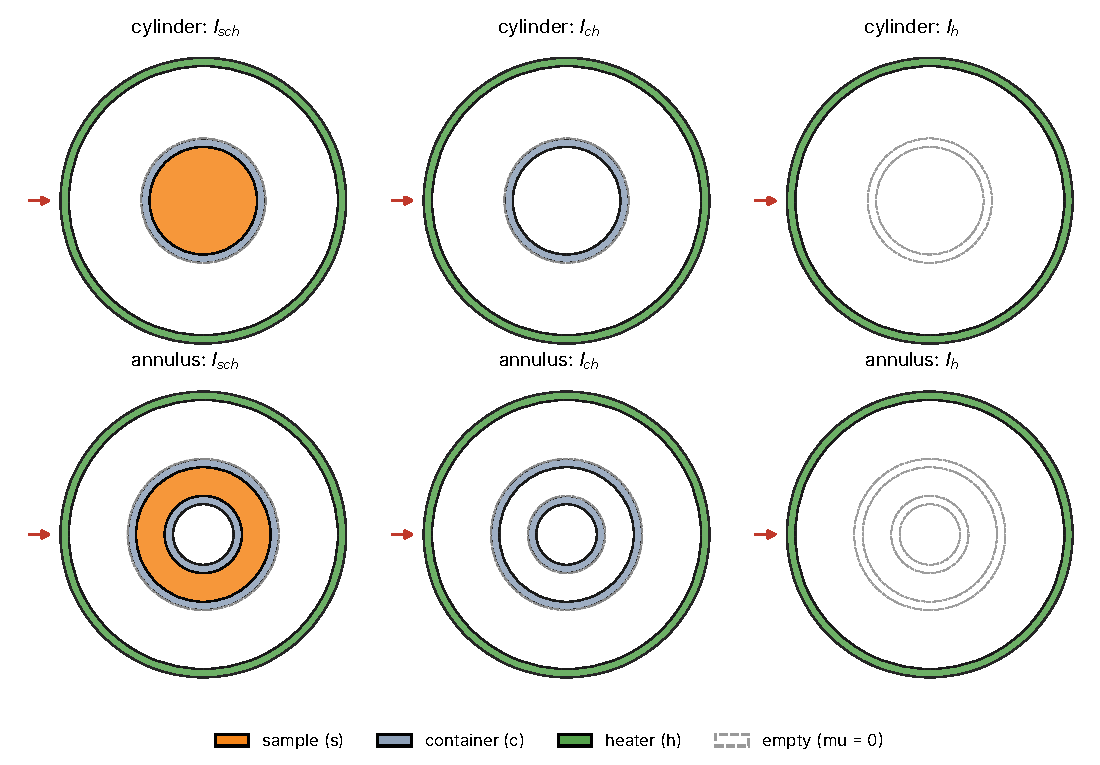
\includegraphics[width=0.92\textwidth]{fig_correct_configs}
  \caption{Top view of the three samples of the two cylindrical examples (radii not to scale). Top: sample in a can inside a
  furnace (Example~13). Bottom: annular sample between two tubes inside a furnace (Example~14). Dashed rings are empty layers
  ($\mu=0$): the geometry is the same in the three runs.}
  \label{fig:correctconfigs}
\end{figure}

\section{The attenuation factors}

The direct method (Chapter~\ref{ch:direct}) gives, for any sample, the single-scattering attenuation factor $A_k(\twotheta)$ of
every layer $k$: particles scattered once in layer $k$, attenuated on the way in and on the way out by all the layers of that sample.
So:
\begin{itemize}
  \item in the \textbf{sch} sample, the factor of the sample layer is $A_{s,sch}$, that of the container layers $A_{c,sch}$, that of the
        heater layers $A_{h,sch}$;
  \item in the \textbf{ch} sample, the container layers give $A_{c,ch}$ and the heater layers $A_{h,ch}$;
  \item in the \textbf{h} sample, the heater layers give $A_{h,h}$.
\end{itemize}
When a part has several layers, its factor is the average of the factors of its layers, weighted by how much each one scatters:
\begin{equation}
  A_{x,y} = \frac{\sum_{k\in x} w_k\, A_k}{\sum_{k\in x} w_k}, \qquad w_k = f_k\,\mu_k\,\langle L_k\rangle ,
  \label{eq:weights}
\end{equation}
where $f_k$ is the scatter fraction, $\mu_k$ the attenuation coefficient and $\langle L_k\rangle$ the mean path of the beam in the
layer. This is because the measured $I_c$ is the sum of the scattering of all the container layers, each one with its own
attenuation. The function \code{attenuation_factors} does all this:
\begin{lstlisting}
from correct_tools import attenuation_factors
A, err, mean_path = attenuation_factors(samples, roles, beam_width=10.0, beam_height=20.0,
                                        angles_deg=np.arange(0, 181, 10.0))
A["s,sch"], A["c,sch"], A["h,sch"], A["c,ch"], A["h,ch"], A["h,h"]    # arrays over 2theta
\end{lstlisting}
The direct method is used for the factors, rather than the first scatterings of the Monte Carlo, because it is much more precise
for thin layers (container walls, heater foils): every point contributes with its exact attenuation, instead of the few particles that
happen to interact in a 0.1~mm foil. Both give the same factors (Chapter~\ref{ch:direct}); \code{attenuation_factors_mc} can replace the
direct method in \code{attenuation_factors} if you want to check it.

\section{Single, multiple and total scattering}
\label{sec:correct-ms}

The Monte Carlo follows every particle through all its scatterings. For each of the three samples,
\code{transmission_by_last_layer} gives the scattering that reaches the detector at each angle, split into single ($S_y$) and
multiple ($M_y$) scattering and by the layer of the last scattering. Divided by $4\pi$ and by the number of incident particles these
are intensities per incident particle and per steradian (isotropic scattering). Their sum $S_y+M_y$ is what the detector measures.
The ratio
\begin{equation}
  \delta_y(\twotheta) = \frac{M_y}{S_y}, \qquad y = sch,\; ch,\; h,
\end{equation}
is the multiple scattering of the whole run: sample, container and heater together, including all the cross terms (a particle
scattered in the sample and then in the heater, and so on).
\begin{lstlisting}
from correct_tools import scattering
sc = scattering(samples, roles, 10.0, 20.0, angles, n_particles=200_000, n_batches=10)
sc["sch"]["single"], sc["sch"]["multiple"], sc["sch"]["total"], sc["sch"]["delta"]   # (mean, error)
sc["sch"]["single_by_part"]["c"]       # single scattering whose last event was in the container
\end{lstlisting}
The errors are the standard errors of the mean of the batches. Use at least 10 batches: with 4, for instance, the error estimate is
itself uncertain by a factor of about 2.

\paragraph{The correction.} With the philosophy of \textsc{correct}, but with the factors and the multiple scattering of \mcams:
\begin{enumerate}
  \item remove the multiple scattering from each measured intensity:
        $I_y^{(1)} = I_y / (1+\delta_y)$, for $y = sch,\,ch,\,h$;
  \item apply the Paalman \& Pings subtraction, eq.~(\ref{eq:pp-chain}), to $I_{sch}^{(1)}$, $I_{ch}^{(1)}$, $I_h^{(1)}$ with the
        six factors.
\end{enumerate}
\begin{lstlisting}
from correct_tools import correct_chain
I_s, I_c, I_h = correct_chain(I_sch_measured, I_ch_measured, I_h_measured, A,
                              delta={"sch": d_sch, "ch": d_ch, "h": d_h})
\end{lstlisting}
\textsc{correct} does step~2 and then subtracts an analytical $\delta$ from the corrected sample only, computed for an equivalent
homogeneous cylinder. Here every run is corrected with its own simulated multiple scattering, for the real geometry. This removes the
approximations of \textsc{correct} discussed in the comparison report: the empirical series for the higher orders, the neglect of the
angle dependence and of the material outside the beam, and the treatment of the container and environment.

\begin{note}[What delta assumes]
Like the Blech \& Averbach correction, $\delta_y$ is computed for \emph{isotropic} scattering in every layer (or for the angular
distribution given with \code{deflection_sampler}). For a sample with strong Bragg peaks or a strongly structured $S(Q)$ this is an
approximation, the same one made by \textsc{correct}. The attenuation factors do not depend on it.
\end{note}

\paragraph{The closure test.} Each example ends with a test of the whole procedure. The simulated totals $S_y+M_y$ are treated as
measurements and corrected with steps~1 and~2. The result must be the true unattenuated scattering of each part,
$I_x = \sum_{k\in x} f_k\mu_k\langle L_k\rangle/(4\pi)$ (function \code{unattenuated}). Because $\delta_y$ comes from the same
simulation, step~1 gives back exactly the simulated single scattering: the test checks the attenuation factors against the Monte
Carlo and the bookkeeping of the subtraction, not the multiple scattering itself. The last column shows what is left when the multiple
scattering is \emph{not} removed. The reference $I_x$ needs the mean paths $\langle L_k\rangle$, which are estimated by sampling; in a
furnace most of the volume is empty and this estimate has an error of a few 0.1\%, so it is averaged over 10 runs and its error is
included. The correction itself does not need $\langle L_k\rangle$.

\section{The helper functions}

\begin{fnbox}{correct\_samples(make, layers, roles, runs=("sch", "ch", "h"))}
The samples of the chosen runs (default the three of \textsc{correct}; \code{RUNS} for all seven) with the same geometry. \code{make(layers)} builds a sample (any geometry).
\code{configuration(layers, roles, measurement)} gives the layers of one of them.
\end{fnbox}
\begin{fnbox}{attenuation\_factors(samples, roles, beam\_width, beam\_height, angles\_deg, n\_points=100000, rng=1)}
The six factors (direct method), their errors, and the mean paths of the layers. Parts with several layers are combined with
eq.~(\ref{eq:weights}).
\end{fnbox}
\begin{fnbox}{scattering(samples, roles, beam\_width, beam\_height, angles\_deg, n\_particles=200000, n\_batches=10, rng=2)}
Single, multiple and total scattering and $\delta$ of the three runs, per incident particle and per steradian, with errors; also split by
the part of the last scattering, and the results of every batch.
\end{fnbox}
\begin{fnbox}{correct\_chain(I\_sch, I\_ch, I\_h, A, delta=None)}
Steps 1 and 2 above: returns the unattenuated $I_s$, $I_c$, $I_h$.
\end{fnbox}
\begin{fnbox}{unattenuated(sample, roles, beam\_width, beam\_height, n\_runs=10)}
True unattenuated single scattering of each part, and its relative error (reference of the closure test, absolute level).
\end{fnbox}
\begin{fnbox}{all\_attenuation\_factors(make, layers, roles, beam\_width, beam\_height, angles\_deg, n\_points=100000, rng=1)}
The 21 factors $A_{x,y}$ for the seven sets of parts (Section~\ref{sec:all-factors}).
\end{fnbox}
\begin{fnbox}{general\_correction(I, A, delta=None, rel\_err=None)}
Unattenuated $I_s$, $I_c$, $I_h$ from any set of runs by weighted least squares, with their errors and $\chi^2$.
\end{fnbox}
\begin{fnbox}{at\_angles(values, angles, new\_angles)}
Linear interpolation of a dict of curves (factors or $\delta$) onto other angles: the angles of the simulated runs, or of the data.
\end{fnbox}
\begin{fnbox}{print\_factors, print\_all\_factors, print\_scattering, print\_contributions, check\_closure, plot\_correct, plot\_all\_factors}
Tables of the results, the closure test, and the figure with the six factors and the three $\delta$.
\end{fnbox}

In all the examples the container and the heater are vanadium ($\mu = 0.0459$~mm$^{-1}$, scatter fraction 0.78), the sample is Ni powder
($\mu = 0.180$~mm$^{-1}$, scatter fraction 0.94, the values of the comparison report at $\lambda = 0.5$~\AA), and the beam is
$10\times20$~mm. The factors are computed every $1^\circ$ and the simulated runs every $2^\circ$ (Section~\ref{sec:grid}).

\subsection*{The angular grid}
\label{sec:grid}
The two calculations do not cost the same per angle. The direct method computes, for every point, the path towards each detector
angle; the Monte Carlo does it for every scattering event of every particle. For the furnace of Example~13 (one run):
\begin{center}\small
\begin{tabular}{@{}rrrr@{}}
  \toprule \textbf{step} & \textbf{angles} & \textbf{factors, direct method ($10^5$ points per layer)} & \textbf{$\delta$, Monte Carlo ($10\times2\times10^5$ particles)} \\ \midrule
  $10^\circ$ & 19 & 17~s & 22~s \\
  $5^\circ$ & 37 & 26~s & 38~s \\
  $2^\circ$ & 91 & 53~s & 83~s \\
  $1^\circ$ & 181 & 99~s & 169~s \\ \bottomrule
\end{tabular}
\end{center}
The factors have sharp features (the dips of the heater factors at $0^\circ$ and $180^\circ$, the collapse of plates near their grazing
angle), so they are computed every $1^\circ$. The multiple-scattering ratio $\delta$ varies slowly, so the Monte Carlo runs every $2^\circ$
and its results are interpolated (function \code{at_angles}, linear interpolation with \code{np.interp}) wherever they are needed on
the $1^\circ$ grid; the closure tests use the factors at the $2^\circ$ angles. With this choice an example with three runs takes 7--11~minutes
(22 for the annulus, which has six layers), and Example~18 (seven runs) about 20, on one processor core. Computing everything every $1^\circ$ would double the time
of the Monte Carlo for no visible gain.

% -------------------------------------------------------------------------
\section{Example 13: cylinder in a can inside a furnace}

Ni powder of 6~mm diameter in a V can (wall 0.2~mm), inside a cylindrical V heater of radius 15~mm (0.1~mm), all 40~mm high; the beam
($20$~mm high) only sees the middle of the sample.

\pyexample{ex13_correct_cylinder}

\begin{figure}[H]
  \centering
  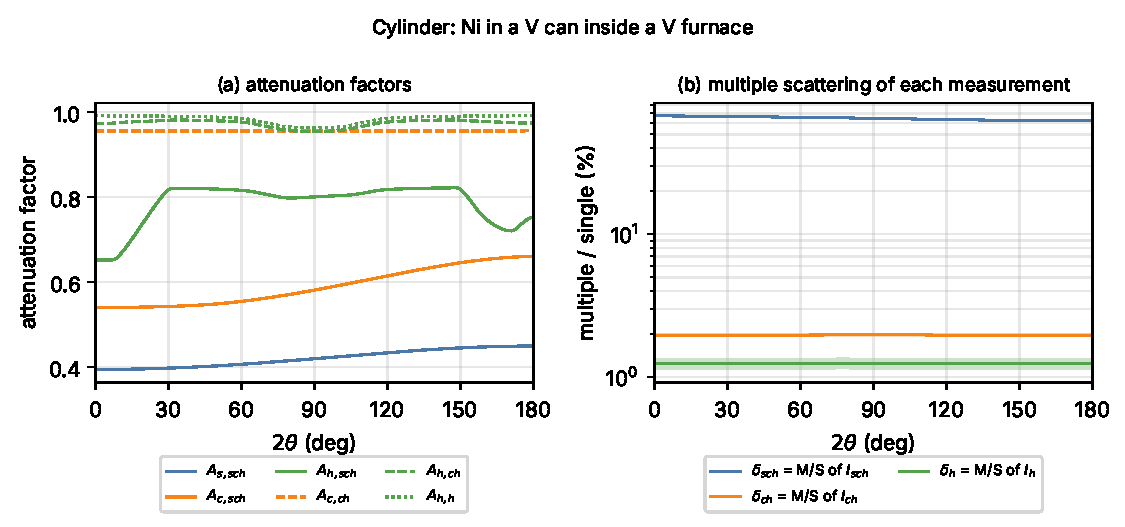
\includegraphics[width=\textwidth]{fig_correct_cylinder}
  \caption{Example 13. (a)~The six attenuation factors. (b)~$\delta=M/S$ of the three runs (log scale) (factors every $1^\circ$, $\delta$ every $2^\circ$ with its statistical error).}
  \label{fig:correctcyl}
\end{figure}

\begin{itemize}
  \item $A_{s,sch}$ goes from 0.394 at $0^\circ$ to 0.449 at $180^\circ$. $A_{c,sch}$ is lower than $A_{c,ch}$ (0.54--0.66 against 0.955):
        the particles scattered in the can cross the sample.
  \item $A_{h,sch}$ has dips at $0^\circ$ and $180^\circ$ (0.65 and 0.75 against about 0.82 elsewhere): there the particles
        scattered in the heater on the beam line cross the sample on their way to the detector. These are the dips that the
        parabolic interpolation of \textsc{correct} misses (comparison report).
  \item $A_{h,ch}$ and $A_{h,h}$ have a dip at $90^\circ$: particles scattered towards $90^\circ$ in the heater wall travel along it.
  \item The multiple scattering of the sample run is large, $\delta_{sch} = 0.67$--0.62 (it decreases with the angle). That of the
        empty can and of the heater is 2\% and 1.2\%.
  \item 94\% of the single scattering of $I_{sch}$ comes from the sample, 4\% from the can, 2--3\% from the heater; of the multiple
        scattering, 97\% ends in the sample.
  \item Closure: the sample is recovered within $0.1\% \pm 0.15\%$, the can and the heater within their statistical errors
        (about 0.9\%). Without the multiple-scattering correction the sample would be 66--71\% too high.
\end{itemize}

% -------------------------------------------------------------------------
\section{Example 14: annular sample between two tubes}

The sample fills the annulus between two coaxial V tubes. From the axis: an empty inner cylinder of 4~mm diameter (role \code{"-"}),
the inner V tube (0.2~mm), the Ni annulus (1.5~mm), the outer V tube (0.2~mm), vacuum, and the V heater at 15~mm. The two tubes
form the container: both have the role \code{"c"}, and their factors are combined with eq.~(\ref{eq:weights}).

\pyexample{ex14_correct_annulus}

\begin{figure}[H]
  \centering
  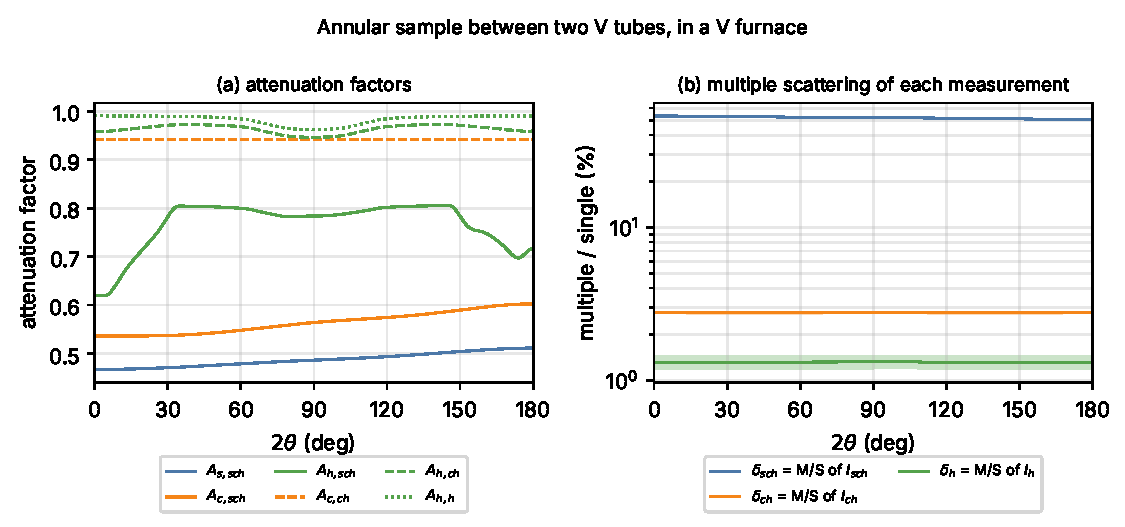
\includegraphics[width=\textwidth]{fig_correct_annulus}
  \caption{Example 14, annular sample. (a)~The six attenuation factors. (b)~$\delta$ of the three runs (factors every $1^\circ$, $\delta$ every $2^\circ$ with its statistical error).}
  \label{fig:correctann}
\end{figure}

\begin{itemize}
  \item The annular sample attenuates less than the full cylinder of Example~13 ($A_{s,sch}$ from 0.467 to 0.511) and has less multiple
        scattering ($\delta_{sch} = 0.53$--0.51), because it is thinner.
  \item The container now has two walls, with more material: $A_{c,ch} = 0.942$ and $\delta_{ch} = 2.8\%$; it gives 6\% of the single
        scattering of $I_{sch}$.
  \item Closure: sample within 0.1--0.3\% (errors 0.1\%), container and heater within their errors.
\end{itemize}
The same layout describes any coaxial assembly: a sample in a double-walled can, a cryostat with several shields (each shield is a
layer with the role \code{"h"}), a container inside a radiation shield, and so on.

% -------------------------------------------------------------------------
\section{Example 15: flat cell between flat heater windows (slab)}

A flat V cell (windows of 0.2~mm, 2~mm of Ni between them) between two flat V heater windows (0.1~mm), 10~mm in front of and behind
the cell, all $40\times40$~mm and perpendicular to the beam. The layers go from the front to the back; the two cell windows have the
role \code{"c"}, the two heater windows the role \code{"h"}. \code{z_front} puts the middle of the Ni on the rotation axis.

\pyexample{ex15_correct_slab}

\begin{figure}[H]
  \centering
  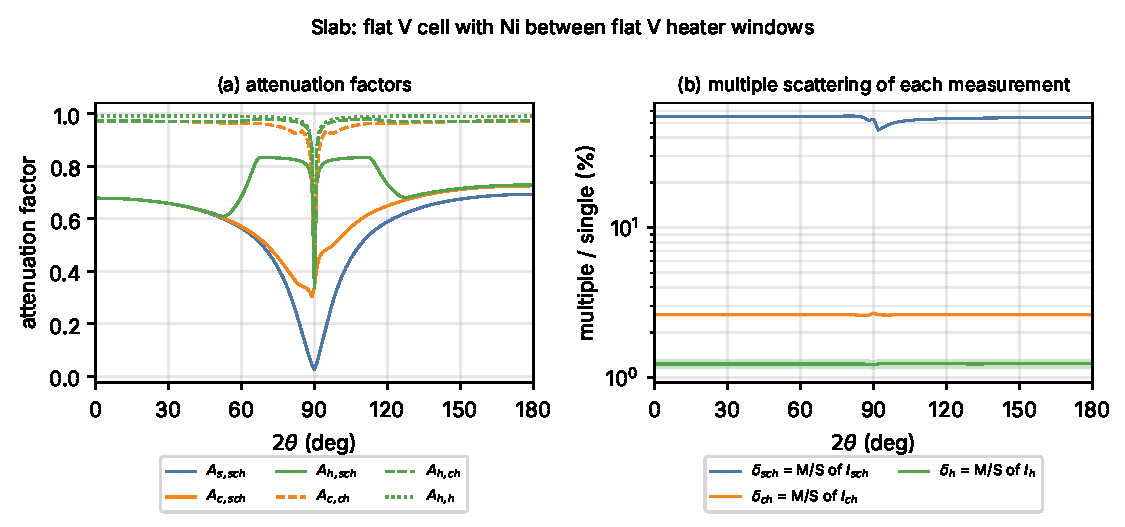
\includegraphics[width=\textwidth]{fig_correct_slab}
  \caption{Example 15, flat cell perpendicular to the beam. (a)~The six attenuation factors. (b)~$\delta$ of the three runs (factors every $1^\circ$, $\delta$ every $2^\circ$ with its statistical error).}
  \label{fig:correctslab}
\end{figure}

\begin{itemize}
  \item At $0^\circ$ every particle leaves along the beam line and crosses the whole stack, whatever layer it was scattered in: the three
        factors of $I_{sch}$ are equal, $\e^{-\sum\mu_k t_k} = 0.6787$. Likewise $A_{c,ch} = A_{h,ch} = \e^{-0.0459\times0.6} = 0.9728$
        and $A_{h,h} = \e^{-0.0459\times0.2} = 0.9909$. These are exact values, reproduced to the fourth decimal.
  \item At $90^\circ$ the scattered particles travel in the plane of the plate: the factors fall (0.026 for the sample) and this angle
        cannot be corrected in practice. Around it the factors change quickly; use a fine grid of angles there, or avoid it.
  \item $\delta_{sch} = 0.53$--0.55: a flat sample much wider than its thickness has a lot of multiple scattering in its plane.
        \textsc{correct} has no multiple-scattering correction for plates.
  \item Closure: sample within 0.1\% (0.3\% at $90^\circ$, error 0.5\%), container and heater within their errors.
\end{itemize}

% -------------------------------------------------------------------------
\section{Example 16: round cell between round heater windows (disc)}

The same stack as Example~15 with a circular section of 30~mm (Chapter~\ref{ch:disc}), rotated so that its plane makes $60^\circ$ with
the beam.

\pyexample{ex16_correct_disc}

\begin{figure}[H]
  \centering
  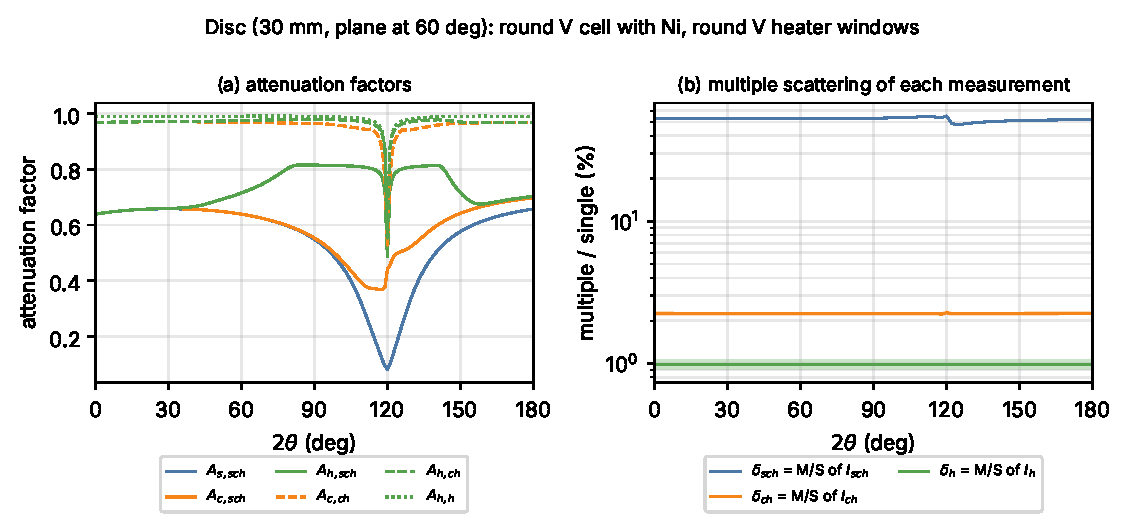
\includegraphics[width=\textwidth]{fig_correct_disc}
  \caption{Example 16, disc at $60^\circ$. (a)~The six attenuation factors. (b)~$\delta$ of the three runs (factors every $1^\circ$, $\delta$ every $2^\circ$ with its statistical error).}
  \label{fig:correctdisc}
\end{figure}

\begin{itemize}
  \item The grazing direction is now at $\twotheta = 180^\circ - 60^\circ = 120^\circ$, where the factors fall (0.082 for the sample).
  \item At $0^\circ$ the three factors of $I_{sch}$ are again equal (0.6393): the beam crosses the tilted stack along a path
        $1/\sin 60^\circ$ times longer, $\e^{-0.3875/0.866} = 0.6393$ ($\sum\mu_k t_k = 0.3875$). At $30^\circ$ the scattered particles leave along the normal of
        the disc, and the factors (0.659) equal those of the plate perpendicular to the beam at $30^\circ$ (Example~15): the incoming and
        outgoing paths are exchanged.
  \item Near the grazing angle the heater and the container give a larger share of $I_{sch}$ (26\% of the single scattering at
        $120^\circ$ against 6\% elsewhere): there the sample hides itself.
  \item Closure: all parts within their errors.
\end{itemize}

% -------------------------------------------------------------------------
\section{Example 17: sphere in a spherical container and heater}

A Ni sphere of 6~mm diameter in a V shell (0.2~mm), inside a spherical V heater of radius 15~mm (0.1~mm), all concentric
(Chapter~\ref{ch:sphere}).

\pyexample{ex17_correct_sphere}

\begin{figure}[H]
  \centering
  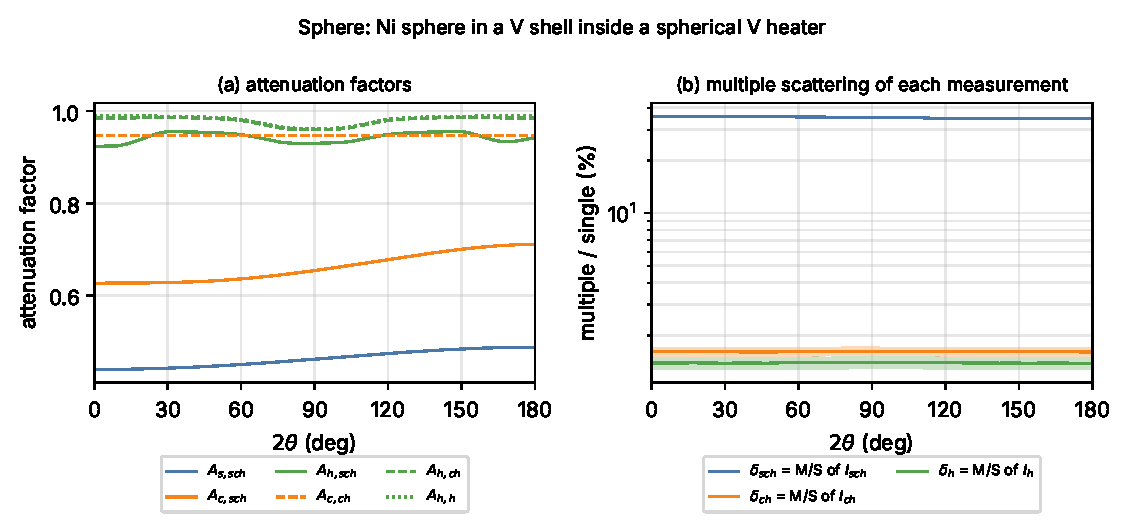
\includegraphics[width=\textwidth]{fig_correct_sphere}
  \caption{Example 17, sphere. (a)~The six attenuation factors. (b)~$\delta$ of the three runs (factors every $1^\circ$, $\delta$ every $2^\circ$ with its statistical error).}
  \label{fig:correctsphere}
\end{figure}

\begin{itemize}
  \item The sphere attenuates less than the cylinder of the same diameter in Example~13: $A_{s,sch} = 0.439$--0.487 against
        0.394--0.449, because its paths are shorter (Chapter~\ref{ch:sphere}). Its multiple scattering is also smaller,
        $\delta_{sch} = 0.36$--0.35 against 0.67--0.62.
  \item The sphere is small compared with the beam ($10\times20$~mm): most of the beam only crosses the heater, which gives 14\% of the
        single scattering of $I_{sch}$. The subtraction of the heater is important here.
  \item $A_{h,sch}$ is close to 1 (0.92--0.96): few of the particles scattered in the heater cross the small sample.
  \item Closure: sample within $0.4\% \pm 0.35\%$; the V shell, a very small volume, has a statistical error of 2\% in the simulated
        intensities (but its factors, from the direct method, are precise to 0.15\%).
\end{itemize}

% -------------------------------------------------------------------------
\section{All the factors $A_{x,y}$, and corrections with any set of runs}
\label{sec:all-factors}

A part $x$ (sample, container or heater) and a set $y$ of parts in the beam (one of the seven runs s, c, h, sc, sh, ch, sch) give
21 factors $A_{x,y}$:
\begin{center}\small
\begin{tabular}{@{}lccccccc@{}}
  \toprule & $y=$ s & c & h & sc & sh & ch & sch \\ \midrule
  $x=$ s & $A_{s,s}$ & $A_{s,c}^{*}$ & $A_{s,h}^{*}$ & $A_{s,sc}$ & $A_{s,sh}$ & $A_{s,ch}^{*}$ & $A_{s,sch}$ \\
  $x=$ c & $A_{c,s}^{*}$ & $A_{c,c}$ & $A_{c,h}^{*}$ & $A_{c,sc}$ & $A_{c,sh}^{*}$ & $A_{c,ch}$ & $A_{c,sch}$ \\
  $x=$ h & $A_{h,s}^{*}$ & $A_{h,c}^{*}$ & $A_{h,h}$ & $A_{h,sc}^{*}$ & $A_{h,sh}$ & $A_{h,ch}$ & $A_{h,sch}$ \\ \bottomrule
\end{tabular}
\end{center}
Do they all make sense? They fall into two groups.

\paragraph{$x$ in $y$: 12 correction factors.} The scattering part is in the beam and attenuates its own scattering. Each of these
factors is needed by some set of runs: the set decides which factors enter the equations
\begin{equation}
  I_y = \sum_{x\in y} A_{x,y}\, I_x \qquad\text{(one equation per run, single scattering)}.
  \label{eq:general}
\end{equation}
\begin{center}\small
\begin{tabular}{@{}>{\raggedright\arraybackslash}p{4.6cm}>{\raggedright\arraybackslash}p{2.0cm}>{\raggedright\arraybackslash}p{7.6cm}@{}}
  \toprule \textbf{Experiment} & \textbf{Runs} & \textbf{Factors} \\ \midrule
  sample in a container in a furnace (\textsc{correct}) & sch, ch, h & $A_{s,sch}$, $A_{c,sch}$, $A_{h,sch}$, $A_{c,ch}$, $A_{h,ch}$, $A_{h,h}$ \\
  sample in a container, no environment & sc, c & $A_{s,sc}$, $A_{c,sc}$, $A_{c,c}$ \\
  self-supporting sample in a furnace & sh, h & $A_{s,sh}$, $A_{h,sh}$, $A_{h,h}$ \\
  self-supporting sample, no environment & s & $A_{s,s}$ \\
  more runs than unknowns, e.g.\ sch, sc, ch, c, h & 5 runs & all the factors of these runs (least squares, below) \\ \bottomrule
\end{tabular}
\end{center}

\paragraph{$x$ not in $y$: 9 diagnostic factors} (marked $^{*}$). The scattering part is not in the beam, so it cannot scatter: these
factors never enter a correction. They can still be defined, as the attenuation of the scattering of $x$ by the \emph{other} parts only.
For example $A_{s,ch}$ is the attenuation, by the container and the heater, of particles scattered at the sample positions, as if the
sample were transparent. They answer two questions:
\begin{itemize}
  \item \emph{How is the attenuation shared between the parts?} For instance $A_{s,h}$ tells how much the heater alone attenuates the
        scattering of the sample.
  \item \emph{Can the factors be multiplied?} One is tempted to write $A_{s,sch}\approx A_{s,s}\,A_{s,c}\,A_{s,h}$ or
        $A_{s,sch}\approx A_{s,s}\,A_{s,ch}$. This is exact only if the attenuation by the other parts is the same for every point of
        $x$ (for instance for an infinite plate at $\twotheta=0$). In general it is not: the product of averages is not the average of
        the product. The diagnostic factors show how large the error is (Example~18).
\end{itemize}

\paragraph{How MCAMS computes the 21 factors.} For the factors with $x$ in $y$ nothing new is needed: the direct method on the sample of
run $y$. For $x$ not in $y$ the layers of $x$ are made \textbf{ghosts}: they keep their geometry but get a vanishing attenuation coefficient,
$\mu = 10^{-12}$~mm$^{-1}$ (\code{GHOST_MU}). The direct method then draws points in them, and their factor is the attenuation by the
parts that are present (a ghost attenuates by less than $10^{-10}$). In practice one sample per run $y$ is built, with the parts of $y$ real
and the others ghosts, and one direct-method run gives the factors of the three parts. Seven runs give the 21 factors:
\begin{lstlisting}
from correct_tools import all_attenuation_factors, print_all_factors
A, err = all_attenuation_factors(MAKE, layers, roles, 10.0, 20.0, angles)
A["s,sch"], A["s,sh"], A["c,sc"], A["s,ch"], ...       # 21 arrays over 2theta
\end{lstlisting}
Parts with several layers are combined with eq.~(\ref{eq:weights}), using the weights of the real layers.

\paragraph{Correcting with any set of runs.} Eq.~(\ref{eq:general}) is one linear equation per run, for the unknowns $I_s$, $I_c$,
$I_h$ that appear in the runs. With multiple scattering, $I_y$ is replaced by $I_y/(1+\delta_y)$. The function
\code{general_correction} solves these equations at every angle by weighted least squares (\code{np.linalg.lstsq}), each equation
divided by the error of its run:
\begin{lstlisting}
from correct_tools import general_correction
parts, errors, chi2 = general_correction(
    {"sch": I_sch, "sc": I_sc, "ch": I_ch, "c": I_c, "h": I_h},      # measured runs
    A, delta={"sch": d_sch, ...}, rel_err={"sch": e_sch, ...})
parts["s"], parts["c"], parts["h"]          # unattenuated I_s, I_c, I_h versus angle
\end{lstlisting}
\begin{itemize}
  \item With as many runs as unknowns, organised as in \textsc{correct} (sch, ch, h), the system is triangular and the least squares
        gives exactly the Paalman \& Pings chain (eq.~\ref{eq:pp-chain}).
  \item With more runs than unknowns, every part is determined by several runs: the statistical errors are smaller, and
        $\chi^2$ (the sum of the squared normalised residuals) measures the consistency of the runs. For $n_y$ runs and $n_x$ unknowns
        it should be about $n_y-n_x$. A much larger value means that something is wrong: a container not put back at the same place,
        a wrong $\mu$, a background not subtracted, a different beam.
  \item The errors of the solution come from the covariance of the least squares, $(M^\mathrm{T}WM)^{-1}$, where $M$ is the matrix of
        the factors and $W$ the weights.
\end{itemize}

% -------------------------------------------------------------------------
\section{Example 18: all the factors, and five sets of runs}

The assembly of Example~13 (Ni in a V can inside a V furnace). The script computes the 21 factors, tests the products, simulates the
seven runs (single and multiple scattering), and corrects them with five different sets of runs.

\pyexample{ex18_all_factors}

\begin{figure}[H]
  \centering
  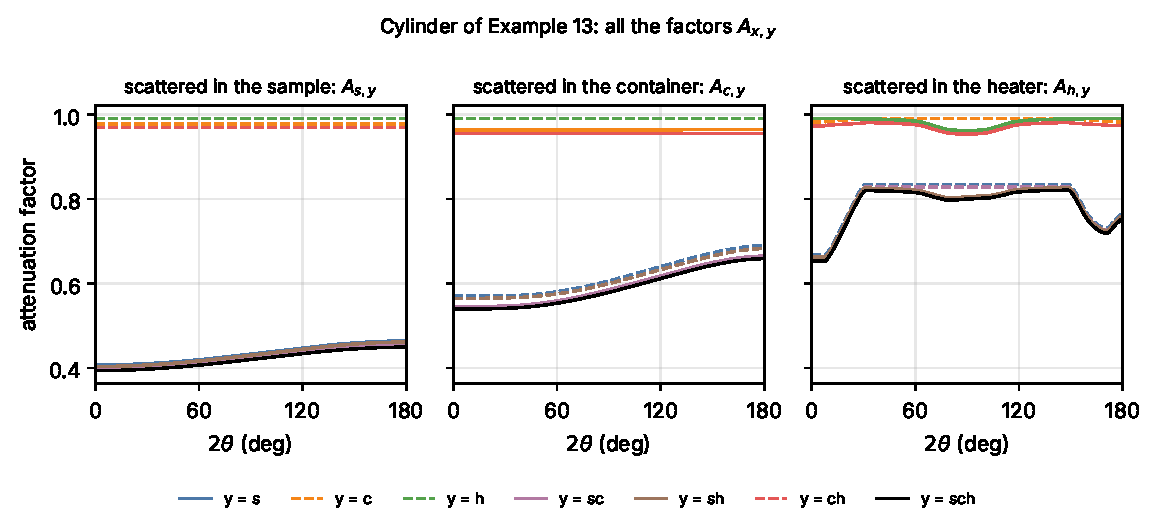
\includegraphics[width=\textwidth]{fig_all_factors_cylinder}
  \caption{Example 18: the 21 factors $A_{x,y}$ versus $\twotheta$ (every $1^\circ$), one panel per scattering part. Solid lines: $x$ in $y$
  (correction factors); dashed: $x$ not in $y$ (attenuation by the other parts only). The line styles of the legend are those of the
  first panel.}
  \label{fig:allfactors}
\end{figure}

\paragraph{The factors.}
\begin{itemize}
  \item The diagnostic factors are close to 1 for thin parts: the can alone attenuates the scattering of the sample by 2.2\%
        ($A_{s,c}=0.978$), the heater alone by 0.9\% ($A_{s,h}=0.991$, two crossings of 0.1~mm of V, $\e^{-0.0459\times0.2}$). The
        sample attenuates the scattering of the can by 30--43\% ($A_{c,s}=0.57$--0.69) and that of the heater most at $0^\circ$
        and $180^\circ$ ($A_{h,s}=0.67$ and 0.77, against 0.83 at $90^\circ$).
  \item \textbf{Products.} For the sample, $A_{s,s}A_{s,c}A_{s,h}$ agrees with $A_{s,sch}$ within 0.2\%, which is the statistical error of
        the comparison: the can and the heater attenuate almost uniformly over the sample. For the container and the heater the
        products are wrong by up to 0.8\% and 1\%: whether a particle scattered in the can or in the heater crosses the sample depends
        strongly on where it was scattered. The factors must therefore be computed for the complete assembly of each run, as done here,
        and not built as products.
  \item The multiple scattering depends little on the container and the heater: $\delta_s = 0.674$, $\delta_{sc}=0.681$,
        $\delta_{sch} = 0.675$ at $0^\circ$.
\end{itemize}

\paragraph{The corrections.} The sample is recovered within 0.1--0.4\% with every set of runs (errors 0.1--0.2\%), and the container and
heater within 1--3 standard errors. With the seven runs together the errors of all three parts are the smallest (0.09\% for the sample),
and $\chi^2$, 2.6--7.2 at the angles shown and 3.9 on average over the 91 angles, for 4 degrees of freedom, shows that the runs are
consistent. With sch, ch, h the least squares and the
Paalman \& Pings chain agree to $6\times10^{-16}$.

\begin{note}[Which factors do I need?]
Only those of the runs you measured: the 12 factors with $x$ in $y$ cover all the usual experiments, and the table above tells which
ones each experiment needs. The other 9 are for understanding the attenuation, not for correcting. If you measured more runs than
strictly needed (for example the empty container with and without the furnace), use them all with \code{general_correction}: you gain
statistics and a consistency test.
\end{note}

% -------------------------------------------------------------------------
\section{Using the factors with measured data}

\begin{enumerate}
  \item \textbf{Describe the assembly} with the real dimensions (mm) and the attenuation coefficients and scatter fractions of the
        materials at the wavelength of the experiment (Chapter~\ref{ch:builder}), and the real beam size and profile.
  \item \textbf{Choose the angles}: factors every $1^\circ$ (or every $2^\circ$ if time matters, with $1^\circ$ near the plane of a plate
        and the dips of the heater factors), $\delta$ every $2$--$5^\circ$ (Section~\ref{sec:grid}).
  \item \textbf{Compute} the factors with \code{attenuation_factors} and $\delta_y$ with \code{scattering}.
  \item \textbf{Interpolate} them onto the angles of the data: \code{at_angles(A, angles, theta_data)} and
        \code{at_angles(delta, angles_mc, theta_data)}.
  \item \textbf{Correct}: background subtraction and normalisation as usual, then \code{correct_chain}; the vanadium used for
        normalisation can be treated in the same way (a sample with its own environment, one more configuration).
\end{enumerate}

\begin{warn}[Statistics]
The factors of the direct method are precise (0.1--0.2\% with $10^5$ points per layer). The Monte Carlo intensities of thin parts
(walls, foils) have errors of 1--2\% with $2\times10^6$ incident particles, because few particles interact there. This is enough for
$\delta_{ch}$ and $\delta_h$, which are small (1--3\%), so their errors are negligible in the corrected data; for the sample,
$\delta_{sch}$ is known to a few 0.1\%. Increase \code{n_particles} or \code{n_batches} if needed.
\end{warn}
